\section{Model matematyczny}
\label{sec:model}

W pierwszej kolejności postanowiono wyznaczyć model matematyczny obiektu sterowania. Dla tego modelu wyznaczane będzie optymalne sterowanie. Podstawową pracą z której korzystano do tego zadania jest \cite{Babazadeh}. Założono, że napęd stanowią silniki prądu stałego. Model takiego silnika w postaci równań stanu można przedstawić w następujący sposób:
\begin{equation}
\begin{aligned}
\dot{x}&=
\begin{bmatrix}
	-\frac{R}{L} & -\frac{k_e}{L} \\
	\frac{k_m}{I_r} & -\frac{k_e}{I_r}
\end{bmatrix}
x+
\begin{bmatrix}
	\frac{1}{L} & 0 \\
	0 & -\frac{1}{I_r}
\end{bmatrix}
u\\
y&=
\begin{bmatrix}
	0 & 1
\end{bmatrix}
x
\end{aligned}
\label{eq:dc_model}
\end{equation}
\noindent gdzie:\newline
\(x=
\begin{bmatrix}
	i \\
	\omega
\end{bmatrix}\) jest wektorem zmiennych stanu\newline
\(i\) jest prądem silnika\newline
\(\omega\) jest prędkością kątową\newline
\(u=
\begin{bmatrix}
	V \\
	\tau
\end{bmatrix}\) jest wektorem sterowań\newline
\(V\) jest napięciem podawanym na silnik\newline
\(\tau\) jest momentem obciążenia mechanicznego\newline
\(I_r\) jest momentem bezwładności przeniesionym na wał silnika\newline
\(L\) jest induktancją\newline
\(R\) jest rezystancją\newline
\(k_e\) jest stałą elektromotoryczną\newline
\(k_r\) jest stałą momentu silnika.

\paragraph*{}
Na rysunku \ref{fig:model_kola} przedstawiono rozkłady sił działających na koła omawianego pojazdu.

\begin{figure}[h]
	\centering
	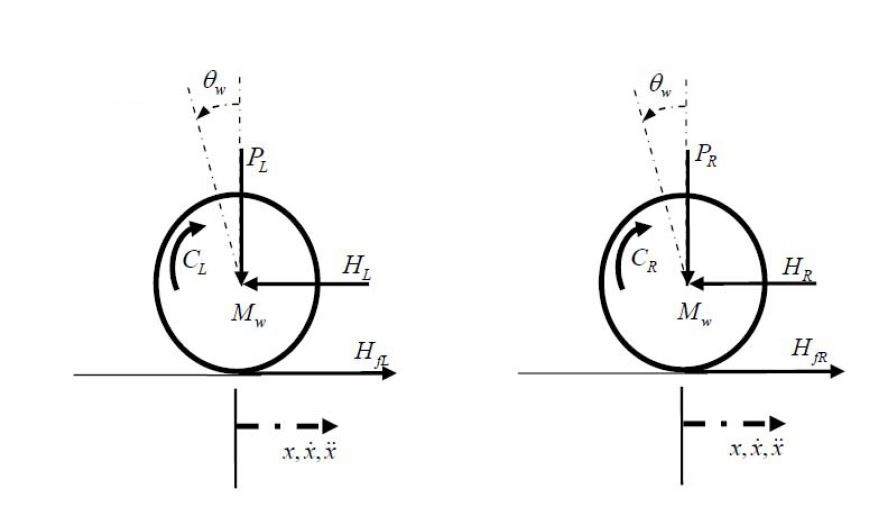
\includegraphics[width=4in]{Figures/model_kola.jpg}
	\captionsource{Siły działające na lewe i prawe koło pojazdu.}{\cite{Babazadeh}}
	\label{fig:model_kola}
\end{figure}

%TODO MK:Dodać wyprowadzenie dynamiki obiektu.

Z drugiego prawa dynamiki Newtona otrzymuje się:
\begin{equation}
\sum F_x=Ma
\end{equation}
\begin{equation}
M_w\ddot x=H_{fR}-H_R
\label{eq:newton_x}
\end{equation}
Z drugiej zasady dynamiki Newtona dla ruchu obrotowego otrzymuje się:
\begin{equation}
\sum M_o=I\alpha
\end{equation}
\begin{equation}
I_w\ddot \theta_w=C_R-H_{fR}r
\label{eq:newton_w}
\end{equation}
Moment silnika DC wynosi:
\begin{equation}
\tau_m=I_R\dot \omega+\tau_a
\label{eq:tau_m}
\end{equation}
Moment przyłożony do kół wynosi:
\begin{equation}
C=I_R\dot \omega=-\frac{k_mk_e}{R}\dot \theta_w+\frac{k_m}{R}V_a
\label{eq:C}
\end{equation}
Równanie \eqref{eq:newton_w} można więc zapisać następująco:
\begin{equation}
I_w\ddot \theta_w=-\frac{k_mk_e}{R}\dot \theta_w+\frac{k_m}{R}V_a-H_{fR}r
\end{equation}
Stąd:
\begin{equation}
H_{fR}=-\frac{k_mk_e}{Rr}\dot \theta_w+\frac{k_m}{Rr}V_a-\frac{I_w}{r}\ddot \theta_w
\label{eq:h_fr}
\end{equation}
Podstawiając \eqref{eq:h_fr} do \eqref{eq:newton_x} otrzymuje się równania dla odpowiednio prawego i lewego koła:
\begin{equation}
M_w\ddot x=-\frac{k_mk_e}{Rr}\dot \theta_w+\frac{k_m}{Rr}V_a-\frac{I_w}{r}\ddot \theta_w-H_R
\label{eq:prawe_w}
\end{equation}
\begin{equation}
M_w\ddot x=-\frac{k_mk_e}{Rr}\dot \theta_w+\frac{k_m}{Rr}V_a-\frac{I_w}{r}\ddot \theta_w-H_L
\label{eq:lewe_w}
\end{equation}
Zakłada się, że nie występuje efekt poślizgu:
\begin{equation}
\ddot \theta_w=\frac{\ddot x}{r}
\label{eq:dd_theta_w}
\end{equation}
\begin{equation}
\dot \theta_w=\frac{\dot x}{r}
\label{eq:d_theta_w}
\end{equation}
Powyższe zależności uwzględnia się we wzorach \eqref{eq:prawe_w} i \eqref{eq:lewe_w}:
\begin{equation}
M_w\ddot x=-\frac{k_mk_e}{Rr^2}\dot x+\frac{k_m}{Rr}V_a-\frac{I_w}{r^2}\ddot x-H_R
\label{eq:prawe_x}
\end{equation}
\begin{equation}
M_w\ddot x=-\frac{k_mk_e}{Rr^2}\dot x+\frac{k_m}{Rr}V_a-\frac{I_w}{r^2}\ddot x-H_L
\label{eq:lewe_x}
\end{equation}
\begin{equation}
2(M_w+\frac{I_w}{r^2})\ddot x=-\frac{2k_mk_e}{Rr^2}\dot x+\frac{2k_m}{Rr}V_a-(H_R+H_L)
\label{eq:total_x}
\end{equation}

\paragraph*{}
Przeanalizować należy również siły działające na użytkownika i drążek sterowania. Zostały one potraktowane jako elementy sztywne. Przedstawiono je na rysunku \ref{fig:model_raczka}.

\begin{figure}[H]
	\centering
	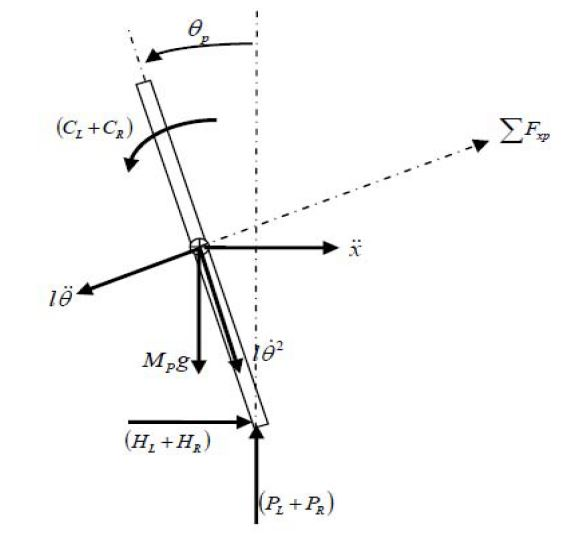
\includegraphics[width=4in]{Figures/model_raczka.jpg}
	\captionsource{Siły działające na pasażera i drążek sterowania.}{\cite{Babazadeh}}
	\label{fig:model_raczka}
\end{figure}

Z drugiej zasadny dynamiki Newtona dla osi x otrzymuje się:
\begin{equation}
\sum F_x=M_p\ddot x
\end{equation}
\begin{equation}
(H_L+H_R)=M_pl\ddot \theta_p\cos \theta_p-M_pl\dot \theta_p^2\sin \theta_p+M_p\ddot x
\label{eq:sum_H}
\end{equation}
Suma sił przyłożonych do drążka i pasażera wynosi:
\begin{equation}
\sum F_{xp}=M_p\ddot x\cos \theta_p
\end{equation}
\begin{equation}
(H_L+H_R)\cos \theta_p+(P_L+P_R)\sin \theta_p-M_pl\ddot \theta_p-M_pg \sin \theta_p=M_p \ddot x \cos \theta_p
\label{eq:sum_forces_rid_hand}
\end{equation}
Moment obrotowy działający na pasażera i drążek względem środka ich masy wynosi:
\begin{equation}
\sum M_o=I\alpha
\end{equation}
\begin{equation}
-(H_L+H_R)l\cos \theta_p+(P_L+P_R)l\sin \theta_p+(C_L+C_R)=I_p\ddot \theta_p
\label{eq:moment_pas_dr}
\end{equation}
Na podstawie równań \eqref{eq:total_x}, \eqref{eq:dd_theta_w} i \eqref{eq:d_theta_w} moment działający na pasażera i drążek wynosi:
\begin{equation}
(C_L+C_R)=-\frac{2k_mk_e}{Rr}\dot x+\frac{2k_m}{R}V_a
\label{eq:sum_C}
\end{equation}
Podstawiając \eqref{eq:C} do \eqref{eq:moment_pas_dr} otrzymuje się:
\begin{equation}
-(H_L+H_R)l\cos \theta_p+(P_L+P_R)l\sin \theta_p+(-\frac{2k_mk_e}{Rr}\dot x+\frac{2k_m}{R}V_a)-I_p\ddot \theta_p
\label{eq:moment_pas_dr_C}
\end{equation}
Po podstawieniu \eqref{eq:sum_forces_rid_hand} do \eqref{eq:moment_pas_dr_C} otrzymuje się:
\begin{equation}
I_p\ddot \theta_p-\frac{2k_mk_e}{Rr}\dot x+\frac{2k_m}{R}V_a+M_pl^2\ddot \theta_p+M_pgl \sin \theta_p=-M_pl\ddot x\cos \theta_p
\end{equation}
Aby wyeliminować \((H_L+H_R)\) z modelu, równanie \eqref{eq:sum_H} podstawia się do równania \eqref{eq:total_x}:
\begin{equation}
2(M_w+\frac{I_w}{r^2})\ddot x=-\frac{2k_mk_e}{Rr^2}+\frac{2k_m}{Rr}V_a-M_pl\ddot \theta_p \cos \theta_p+M_pl\dot \theta_p^2\sin \theta_p-M_p\ddot x
\end{equation}
Na podstawie powyższych wyprowadzeń otrzymano nieliniowe równania dynamiki obiektu:
\begin{equation}
(M_pl^2+I_p)\ddot \theta_p-\frac{2k_mk_e}{Rr}\dot{x}+\frac{2k_m}{R}V_a+M_pgl\sin \theta_p=-M_pl\ddot x\cos \theta_p
\end{equation}
\begin{equation}
\frac{2k_m}{Rr}V_a=(2M_w+\frac{2I_w}{r^2}+M_p)\ddot x+\frac{2k_mk_e}{Rr^2}\dot x+M_pl\ddot \theta_p\cos \theta_p-M_pl\dot \theta_p^2\sin \theta_p
\end{equation}
Równania te przekształcono do postaci nieliniowych równań stanu:
%\begin{equation}
%\begin{aligned}
%\dot x_1 &= x_2\\
%\dot x_2 &= -\frac{a_8}{a_7}x_2-\frac{a_9}{a_7}\dot x_4\cos x_3-\frac{a_{10}}{a_7}x_4^2\sin x_3+\frac{a_6}{a_7}u\\
%\dot x_3 &= x_4\\
%\dot x_4 &= \frac{(a_5a_6\cos x_3-a_3a_7)u-(a_5a_8\cos x_3+a_2a_7)x_2-a_4a_7\sin x_3-a_5a_{10}x_4^2\sin x_3\cos x_3}{a_1a_7+a_5a_9\cos^2 x_3}
%\end{aligned}
%\label{eq:nonlinear_ss}
%\end{equation}
\begin{equation}
\begin{aligned}
\dot x_1 &= x_2\\
\dot x_2 &= k_1x_2+k_2\frac{L(x,u)}{M(x)}\cos x_3+k_3x_4^2\sin x_3+k_4u\\
\dot x_3 &= x_4\\
\dot x_4 &= \frac{L(x,u)}{M(x)}\\
L(x,u) &= (k_5\cos x_3+k_6)u+(k_7\cos x_3+k_8)x_2+k_9\sin x_3+k_{10}x_4^2\sin x_3\cos x_3\\
M(x) &= k_{11}+k_{12}\cos ^2x_3
\end{aligned}
\label{eq:nonlinear_ss}
\end{equation}
\noindent gdzie:\newline
\(k_{1\dots 12}\) są stałymi parametrami obiektu.

\paragraph*{}
Opisany powyżej model zaimplementowano w środowisku programowym \textit{MATLAB}. Został on przetestowany poprzez zadanie takich warunków w których można łatwo przewidzieć zachowanie rzeczywistego obiektu, np. niewielkie odchylenie od niestabilnego punktu równowagi (obiekt ustawiony pionowo do góry). Odpowiedź modelu dla tej sytuacji przedstawiono na rysunku \ref{fig:wychylenie_test}. W tym wypadku odpowiedź obiektu przypomina wahadło fizyczne. Na rysunku \ref{fig:polozenie_test} pokazano jak zmienia się położenie pojazdu w opisywanej sytuacji. Przebiegi czasowe zmiennych stanu zgadzają się z przewidywanym zachowaniem realnego urządzenia (nie biorąc pod uwagę uderzenia w ziemię).
\newpage
\begin{figure}[h]
	\centering
	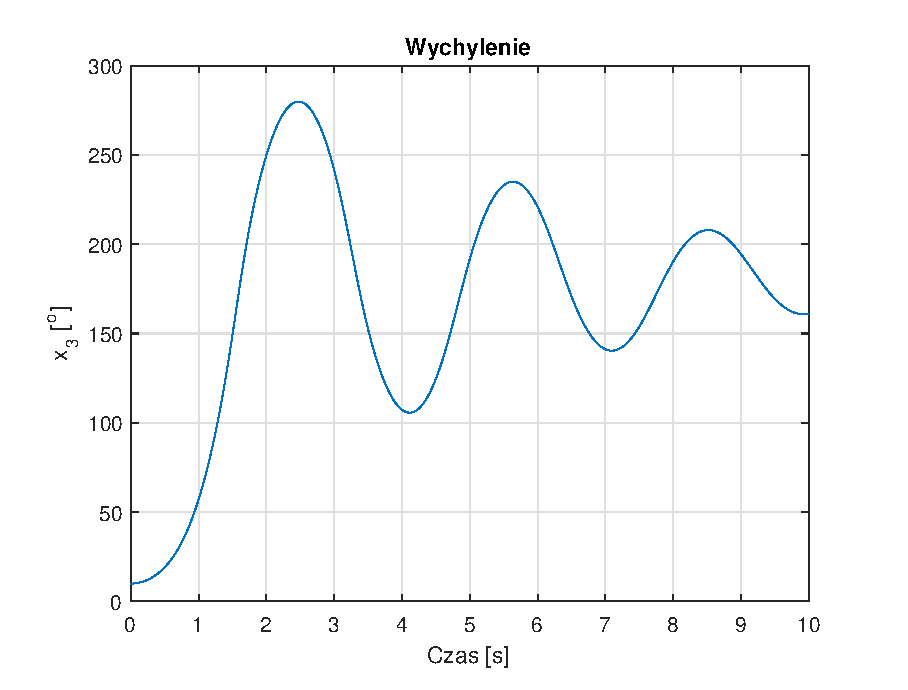
\includegraphics[width=4in]{Figures/wychylenie_test.eps}
	\caption{Wychylenie zmiennej \(x_3\) (kąta) z niestabilnego punktu równowagi.}
	\label{fig:wychylenie_test}
\end{figure}

\begin{figure}[H]
	\centering
	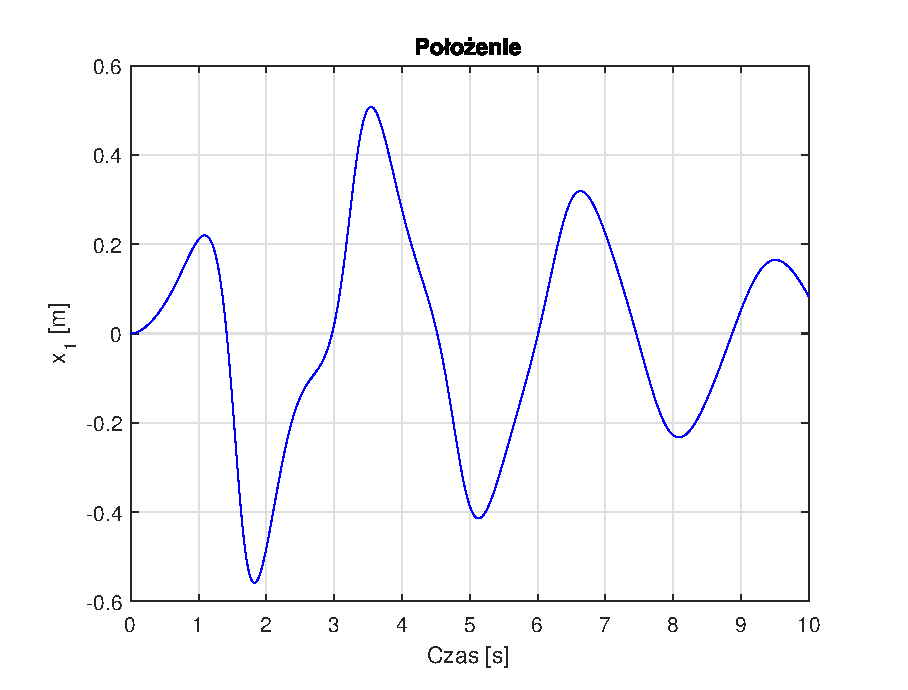
\includegraphics[width=4in]{Figures/polozenie_test.eps}
	\caption{Przebieg zmiennej \(x_1\) (położenia).}
	\label{fig:polozenie_test}
\end{figure}

Postanowiono również porównać zaimplementowaną metodę Rungego-Kutty 4-go rzędu z wbudowaną funkcją \textit{ode45}. Porównanie to dla częstotliwości próbkowania równej 1 kHz przedstawiono na rysunku \ref{fig:wychylenie_1khz}. Natomiast na rysunku \ref{fig:wychylenie_10khz} pokazano to samo porównanie dla częstotliwości próbkowania równej 10 kHz. Różnice pomiędzy tymi metodami są niewielkie. Otrzymane wyniki są prawie takie same również dla zwiększonej częstotliwości próbkowania. Można więc stwierdzić, że częstotliwość 1 kHz jest wystarczająca, do poprawnego modelowania zachowania obiektu.
\newpage
\begin{figure}[h]
	\centering
	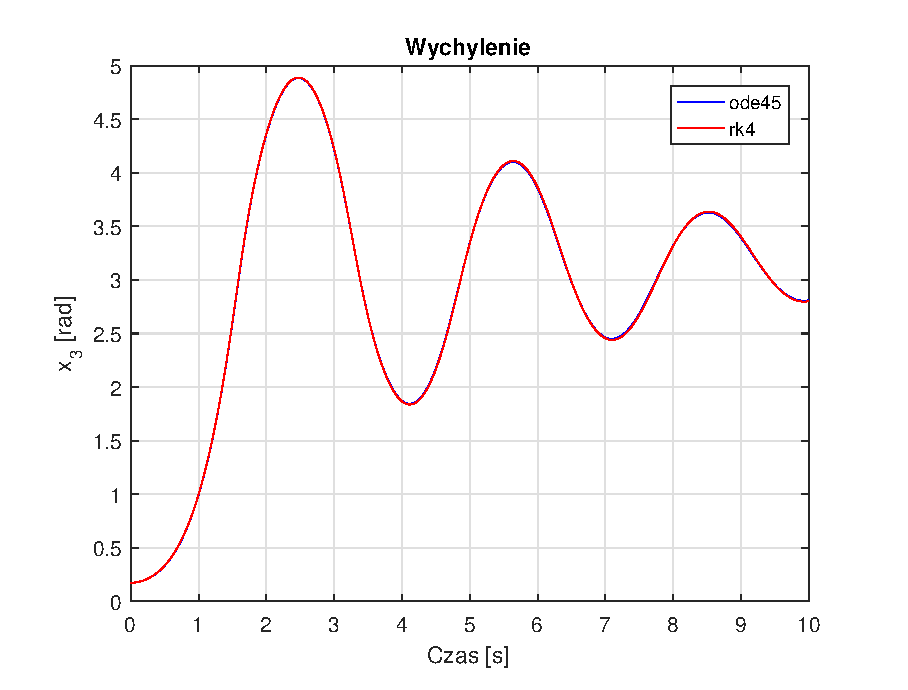
\includegraphics[width=4in]{Figures/wychylenie_1khz.eps}
	\caption{Porównanie dla częstotliwości próbkowania równej 1kHz.}
	\label{fig:wychylenie_1khz}
\end{figure}

\begin{figure}[h]
	\centering
	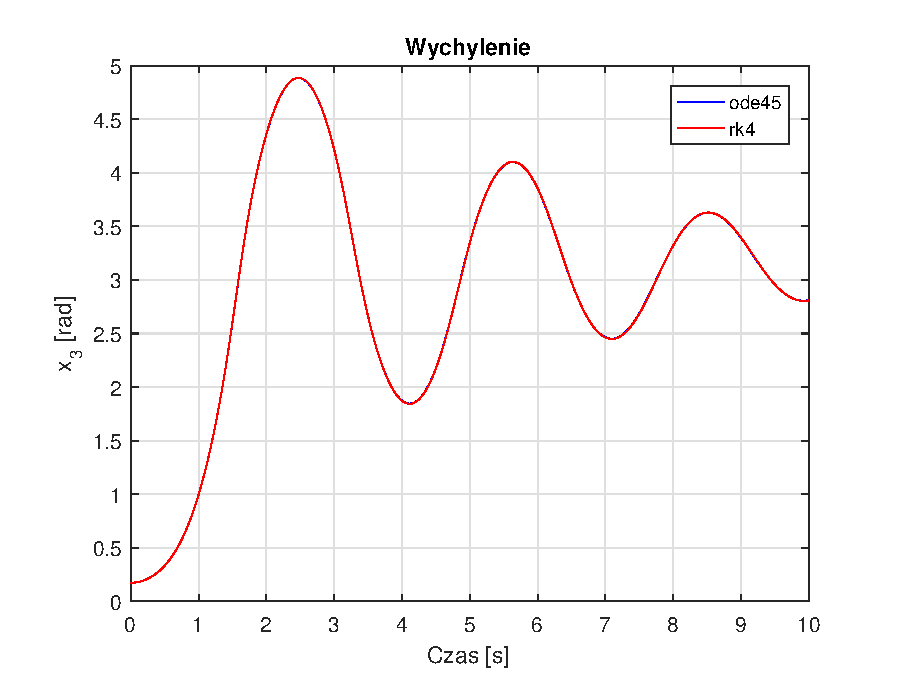
\includegraphics[width=4in]{Figures/wychylenie_10khz.eps}
	\caption{Porównanie dla częstotliwości próbkowania równej 10kHz.}
	\label{fig:wychylenie_10khz}
\end{figure}